			\begin{question}{/}{Trigonométrie}{2}{1217 et 31 et 1213}
				Un vecteur fait un angle de 60 degrés avec l'axe $x$, et a une norme de 6. Quelle est la composante selon $x$ du vecteur?
            \end{question}
            \begin{reponses}
            	\item[false] $3\sqrt{2}$
            	\item[false] 6
                \item[false] $3\sqrt{3}$
                \item[true] 3
            \end{reponses}
			%%%%%%%%%%%%%%%%%%%%%%%%%%%%%%%%%%%%%
            \begin{question}{/}{Trigonométrie}{2}{1217 et 31 et 1213}
                Que valent les coordonnées $x$ et $y$ du vecteur ci-dessous?
                \begin{center}
                	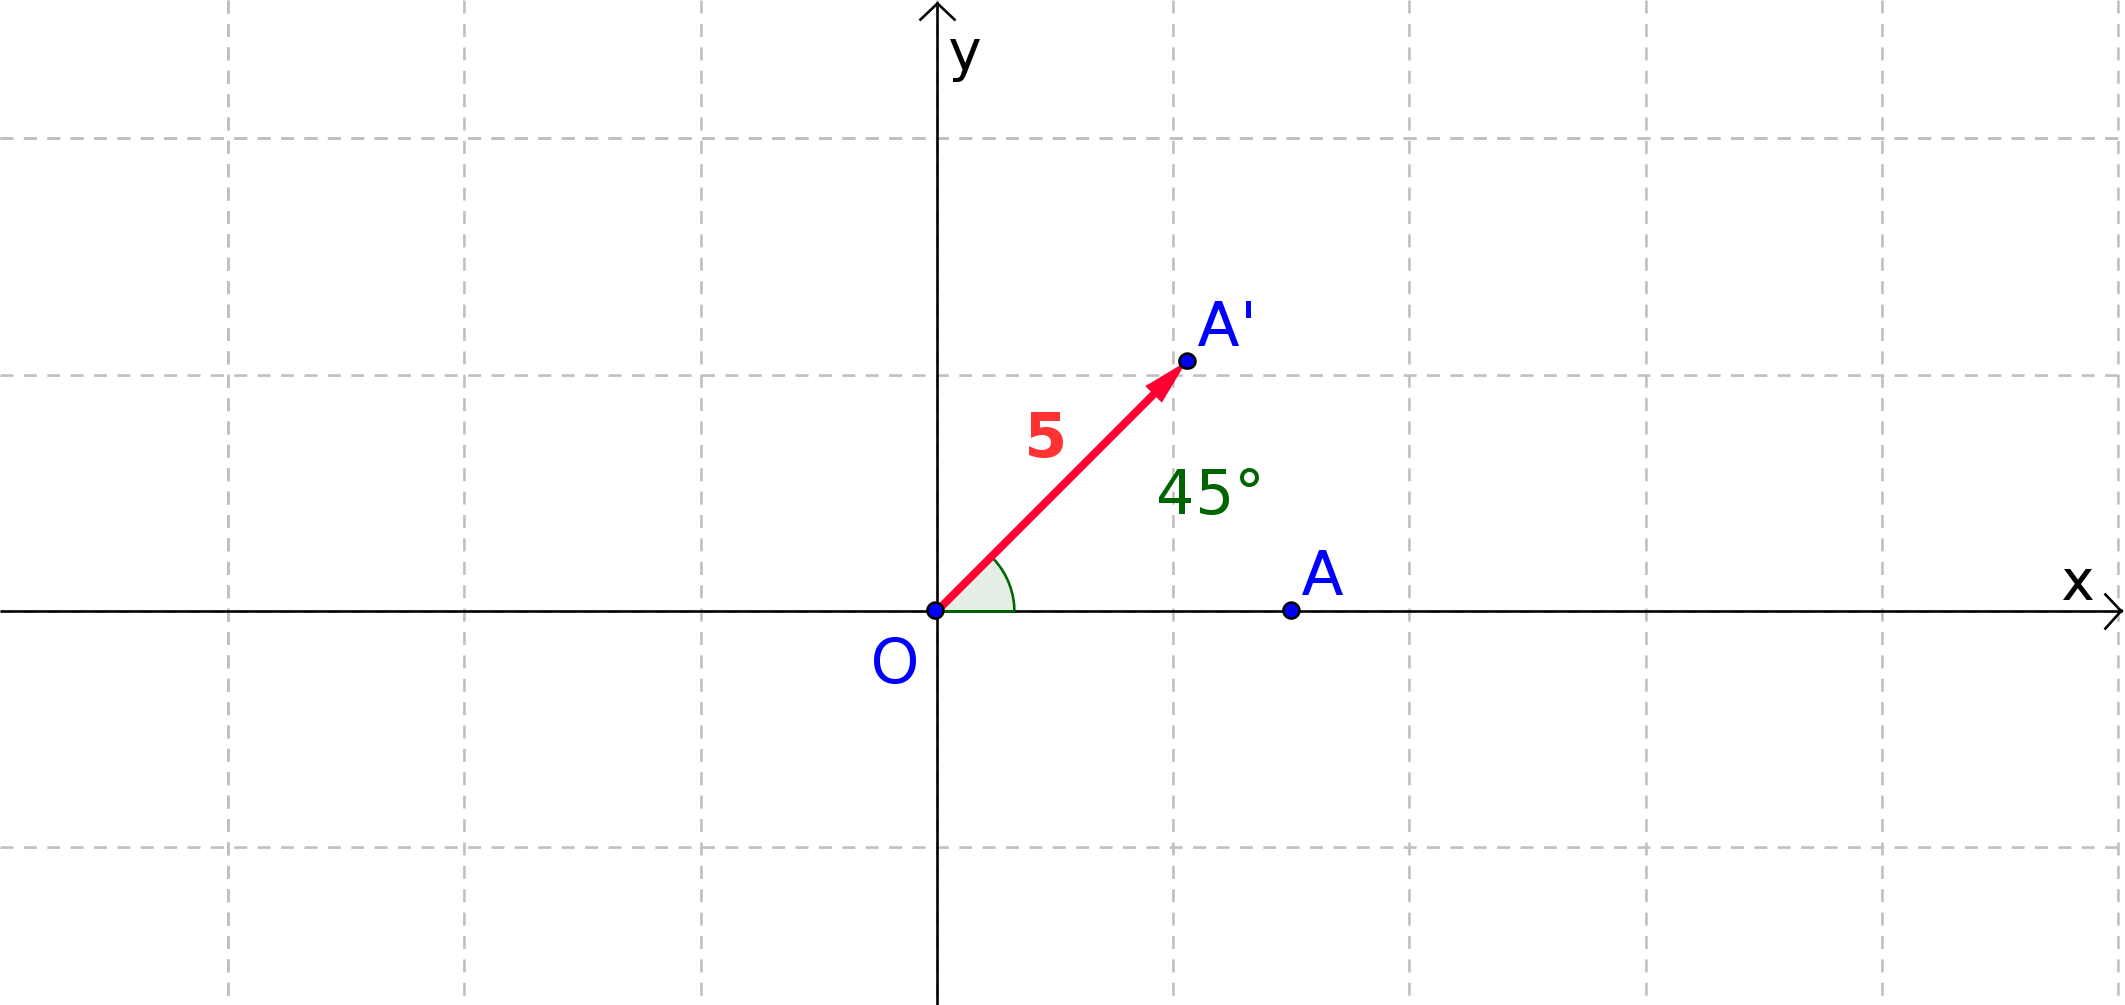
\includegraphics[width=0.5\textwidth]{Philippe/Figures_Philippe/trigo_1_5.png}
                \end{center}
            \end{question}
            \begin{reponses}
                \item[false] $x = \frac{\sqrt{2}}{2}$ et $y = \frac{\sqrt{3}}{2}$
                \item[true] $x = 5\frac{\sqrt{2}}{2}$ et $y = 5\frac{\sqrt{2}}{2}$
                \item[false] $x = 5\frac{\sqrt{3}}{2}$ et $y = \frac{5}{2}$
                \item[false] $x = \frac{\sqrt{3}}{2}$ et $y = \frac{1}{2}$
            \end{reponses}
            %%%%%%%%%%%%%%%%%%%%%%%%%%%%%%%%%%%%%
            \begin{question}{/}{Trigonométrie}{2}{1217 et 31 et 1213}
            	Un objet se déplace avec un angle de 30 degrés par rapport à l'axe horizontal à une vitesse de \SI{10}{\meter\per\second}. Quelle est la valeur de la vitesse de l'objet par rapport à l'axe horizontal?
            \end{question}
            \begin{reponses}
                \item[false] $5\;\si{\meter\per\second}$
                \item[false] $\sqrt{2}/2\;\si{\meter\per\second}$
                \item[false] $\sqrt{3}/2\;\si{\meter\per\second}$
                \item[true] $5\sqrt{3}\;\si{\meter\per\second}$
            \end{reponses}
            %%%%%%%%%%%%%%%%%%%%%%%%%%%%%%%%%%%%%
        	\begin{question}{/}{Trigonométrie}{3}{1217 et 31 et 1213}
				Un vecteur de norme $3$ fait un angle $\theta$ avec l'horizontale. La projection sur l'axe vertical est de $1,5$. Parmis les angles suivant, lequel peut être égal à $\theta$?
            \end{question}
            \begin{reponses}
            	\item[false] $\frac{\pi}{2}$
            	\item[false] $\frac{\pi}{3}$
                \item[false] $\frac{\pi}{4}$
                \item[true] $\frac{\pi}{6}$
            \end{reponses}
			%%%%%%%%%%%%%%%%%%%%%%%%%%%%%%%%%%%%%
            \begin{question}{/}{Trigonométrie}{3}{1217 et 31 et 1213}
                Un pendule de longueur \SI{10}{\centi\meter} forme un angle $\theta$ avec la verticale, de manière à ce que sa projection sur l'axe vertical soit de \SI{5}{\centi\meter}. Que vaut $\theta$?
            \end{question}
            \begin{reponses}
                \item[true] 60 degrés
                \item[false] 30 degrés
                \item[false] 45 degrés
                \item[false] 90 degrés
            \end{reponses}
            %%%%%%%%%%%%%%%%%%%%%%%%%%%%%%%%%%%%%
